\section{Adding Prudence to Process}\label{solution}
Despite the unique attributes about software, the risk of negligence liability
and the cost to defend unavoidable risks can be reduced. We have already
analyzed the properties of software that make it difficult to operate in
safety-critical environments in Section \ref{software_props}. This section
identifies a key process area of software development that needs improvement if
a team is to develop safety-critical software.

Our solution aims to minimize risks in safety-critical software environments and
reduce the cost to defend negligence liabilities in the case of legal disputes.
The documentation process is the key to our solution. Documentation is an
effective way to find bugs in a software program and thoroughly testing it may
be the most cost-effective way to reduce the risk of legal disputes
\cite{Kaner_doc_1995}. The model proposed in this paper introduces an
improvement to the software engineering workflow designed for safety-critical
environments that will provide traceable documentation comments that developers
can use minimize software defects and lawyers can use to defend (or confirm)
negligence.

They premise of our research is predicated on the utility of good documentation
and the foreseeabe habits of software developers. In practice, programmers just
want to write code and do not want to be disturbed by meta-work involving
documentation. But the programmers are the most qualified persons to be writing
comments about an implementation -- they are the ones who are developing it! In
addition, the intended audience of documentation comments is not limited to
other programmers. In the case of a legal dispute, lawyers and analysts will
want access to all forms of documentation, including comments, to interpret the
safety precautions taken by the implementers.

\subsection{Goals}
Software in the safety-critical realm is especially vulnerable to negligence
liabilities. Because of this, we believe that it is in an organization's best
interest to document, or comment, on the activities of the persons doing
safety-critical work. By recording this data in a versioned and traceable 
database, an organization will be able to track and identify the information
that it deems important to a safety-critical project. We put this system into
place, but leave it up to the organization to specify what they need to record
in this database. The design goals for this system are shown in Figure 
\ref{fig:design_criteria}.

\begin{figure}
\makebox[\textwidth]{\hrulefill}
\begin{itemize}
  \item \textbf{Constraints on system}
    \begin{itemize}
      \item allows easy, real-time commenting for developers
      \item comments can be associated with multiple areas of source code
    \end{itemize}
  \item \textbf{Constraints on data representation and implementation}
    \begin{itemize}
      \item integrates commenting capabilities into IDE
      \item documentation comments separated from source code
      \item stores comment versioning and ownership information
      \item indexes comments based on code references, author, version
      \item preserves comment-to-code associations across code changes
    \end{itemize}
\end{itemize}
\makebox[\textwidth]{\hrulefill}
\caption{Design goals for the system}
\label{fig:design_criteria}
\end{figure}

The system constraints define our goals as they are seen by the users of the
system (in this case, the software developers working on a safety-critical
project).There are two defining goals for this system. First, the system must
allow for ``easy'' commenting capabilities in real-time. This means that
developers must be able to easily write free-text prose in a natural language
while they writing code. Also, the comments that the developers produce must be
able to be explicitly associated with multiple lines of code in the source.
These lines can exist in the different functions, classes, and even different
files if necessary. This allows the utilizing organization be very flexible in
specifying what it wants to record.

We also specify constraints on the representation of data and implementation (as
of the time of this paper's writing, a prototype implementaiton has yet to be
built). In order to satisfy the ``easy'' requirement, commenting abilities must
be integrated into the IDE. The next implementation constraint is sufficient for
satisfying the second goal of the system. By physically separating comments from
the source code, we overcome the limiting attributes of traditional comments and
allow the ability to put link associations into place. These associations will
be stored in some sort of database (most likely through a relational database
schema). If this system is to be useful, then an organization must be able to
query this database based on code references, authors of code, or different
versions of the software release. In order to achieve this, the system must
store this informaiton, and maintain it across changes in the code.

\subsection{Comment Classification}

\begin{figure}
\begin{narrow}{-1.5in}{-1.5in}
\begin{center}
\includegraphics[scale=0.75]{images/comments.eps}
\end{center}
\end{narrow}
\caption{Overview of comment-to-code association}
\label{comment_to_code}
\end{figure}

A \textbf{software comment} is a fragment of natural language intended for human
consumption. More formally, a comment is ``\textit{explanatory text embedded in
program source intended to help human readers understand it."} \cite{FOLDOC}.
For the purposes of this research, we distinguish comments into two separate 
classes: 
\begin{enumerate}
  \item code comments
  \item documentation comments
\end{enumerate}

\textbf{Code comments} refer to the in-line comments that programmers write to
describe specific behavior of small snippets of code. In Java or C, these types
of comments are normally preceded by `\verb!//!' or surrounded by a preceding 
`\verb!/*!' and a trailing `\verb!*/!'. \textbf{Documentation comments} refer to
comments used as reference material intended for human consumption to describe 
entire functions, classes, and packages. Javadoc \cite{Javadoc} is a popoular
representation of documentation comments. In Java, they are distinguished by a
preceding `\verb!/**!' and a trailing `\verb!*/!'.

Figure \ref{comment_to_code} shows how our system associates documentation
comments to source code. The source code of the program can still contain inline
code comments to explain quick attributes about the programming techniques in
the direct vicinity of the comment. But documentation comments are stored
separate from the source code. In addition, the author of the comment and the
time it was written are also stored. Association links are created in a
many-to-many fashion. A single comment can be associated with many lines of code
(which do not have to be contiguous lines). In addition, a single line of code
(or an area of code) can be associated with multiple comments.

\subsection{A Prudent Process}

\begin{figure}
\begin{narrow}{-1.25in}{0in}
\begin{center}
\includegraphics[scale=0.75]{images/prudence.eps}
\end{center}
\end{narrow}
\caption{Development phase for safety-critical projects}
\label{prudence}
\end{figure}

